\documentclass[pdftex,a4paper,12pt,onecolumn,fleqn,captions=tableheading]{scrartcl}

\usepackage[british]{babel}
\usepackage[utf8]{inputenc}
%\usepackage[T1]{fontenc}
\usepackage{graphicx}
\usepackage{booktabs}
\usepackage{caption}
\usepackage{subcaption}
\usepackage{lmodern}
\usepackage{microtype}
\usepackage{textcomp}
\usepackage{amssymb}
\usepackage{epstopdf}
\usepackage{capt-of}
\usepackage{amsmath}
\usepackage{float} 
\usepackage{xfrac}
\usepackage{dblfloatfix}

\addtokomafont{caption}{\small}
\setkomafont{captionlabel}{\sffamily\bfseries}


\usepackage[nottoc]{tocbibind}

% page layout
% \usepackage[a4paper,onecolumn]{geometry}
% \geometry{hmargin=50pt,top=60pt,bottom=80pt}
% \geometry{onecolumn,columnsep=20pt}
% \geometry{head=30pt,headsep=30pt,foot=40pt}

% header and footer
% \usepackage{fancyhdr}
% \setlength{\headheight}{15pt}
% \pagestyle{fancy}
%\fancyheadoffset{9pt}
%\fancyfootoffset{9pt}
% \lhead{}	\chead{Arduino - Octave paddle}	\rhead{}
% \lfoot{}	\cfoot{ \\ \thepage}	\rfoot{}
%\renewcommand{\headrulewidth}{0,1 mm}
% \renewcommand{\footrulewidth}{\headrulewidth}

\begin{document}
% top matter
\title{User Manual Wave Tank Actuator v1.0}
\author{J. Rabault, jean.rblt@gmail.com}
\date{\today}

\maketitle

\section{Introduction}

This is a quick user manual describing the functionning, set up and use of the paddle control actuator system to be used in Svalbard. For any complementary question, contact me at: jean.rblt@gmail.com.

\section{General function}

\subsection{Working principle}

A linux computer is used to drive a linear actuator through an Arduino board connected to a motor control shield. The computer sends to the Arduino board the instruction in position (set point) at a rate of 200 Hz through a serial USB connection. The connection to the Arduino and the generation of the set point instruction are done through Octave and the Octave library instrument-control. The Arduino boards receives the set point from the computer and runs internally a PID control loop at a frequency of 500 Hz. The position of the actuator is measured using a LVDT sensor. The Arduino controls the linear actuator through a H-bridge control shield. The components indicated below are the ones used in v1.0. Other similar components could be used.

\subsection{Components}

The components require to build a working system are:

\begin{itemize}
\item A computer running Linux (Ubuntu 14.04 or more recent recommended), on which Octave and its package instrument-control are installed (to be set up by UNIS).
\item A 12V power supply used to power the actuator. The power capability must be adapted to the maximum power of the linear actuator (to be set up by UNIS, recommended 20 Amps capability).
\item An Arduino board on which the custom buffer source code (1024 bits RX buffer) and the Actuation.ino program have been loaded (done at UiO). The Arduino board must be connected by USB to the computer. If long distances are required, use a special USB cable adapted for long distance signal transmission (not tested at UiO).
\item On top of the Arduino, a Mega Moto Plus with the control jumpers configured to match the Arduino.ino program (done at UiO).
\item A LDVT position sensor, connected to the soldered board for acquisition by the Arduino (done at UiO) and to the 12V power supply. The soldered board will be connected on top of the Moto shield.
\item A linear electric actuator (present model: Progressive Automation PA-15-6-11).
\end{itemize}

\subsection{Software}

The program uploaded on the Arduino board is loaded once and for all and implements the PID loop. The only program to be run for controlling the system is the Actuator.m Octave script, together with its sub functions. This script takes care of set point instruction signal generation, serial communication with the board, and collects the information generated by the PID loop. See section ''Octave code''.

\section{System set up and use}

\subsection{Electrical connections}

To set up the system, the following connections must be done:

\begin{itemize}
\item Connection of the Moto Shield to the Arduino: done at UiO, by setting the shield on top of the Arduino board.
\item Connection of the actuator to the Moto shield: connect the power cables from the actuator to the ACT plug on the shield. Respect polarity, i.e. red cable to screw A, black cable to screw B as indicated in figure 1.
\item Connection of the sensor to the Arduino through the Moto shield pints: connect the soldered board on the shield. The pin on the right of the soldered board must correspond with the A5 Arduino pin, as indicated in figure 2.
\item Connection of the Moto shield to the power source: connect the PWR screws to the 12V power supply. Respect polarity, as indicated on figure 1 (red to plus 12V, black to 12V supply ground).
\item Connection of the LVDT sensor to the power source: connect the cables coming out of the soldered board to the 12V power supply. Respect polarity (red to plus 12V, black to 12V supply ground).
\item Connection of the Arduino board to the computer by USB cable. If long distances are requirede, use a special cable.
\end{itemize}

The overall configuration of the system is presented in figure 4. Respect polarity. Polarity inversion of the power supply to the sensor or the Moto shield may damage the components. Polarity inversion of the actuator connection will inverse the displacement direction and make the control loop unstable.

\begin{figure}
\begin{center}
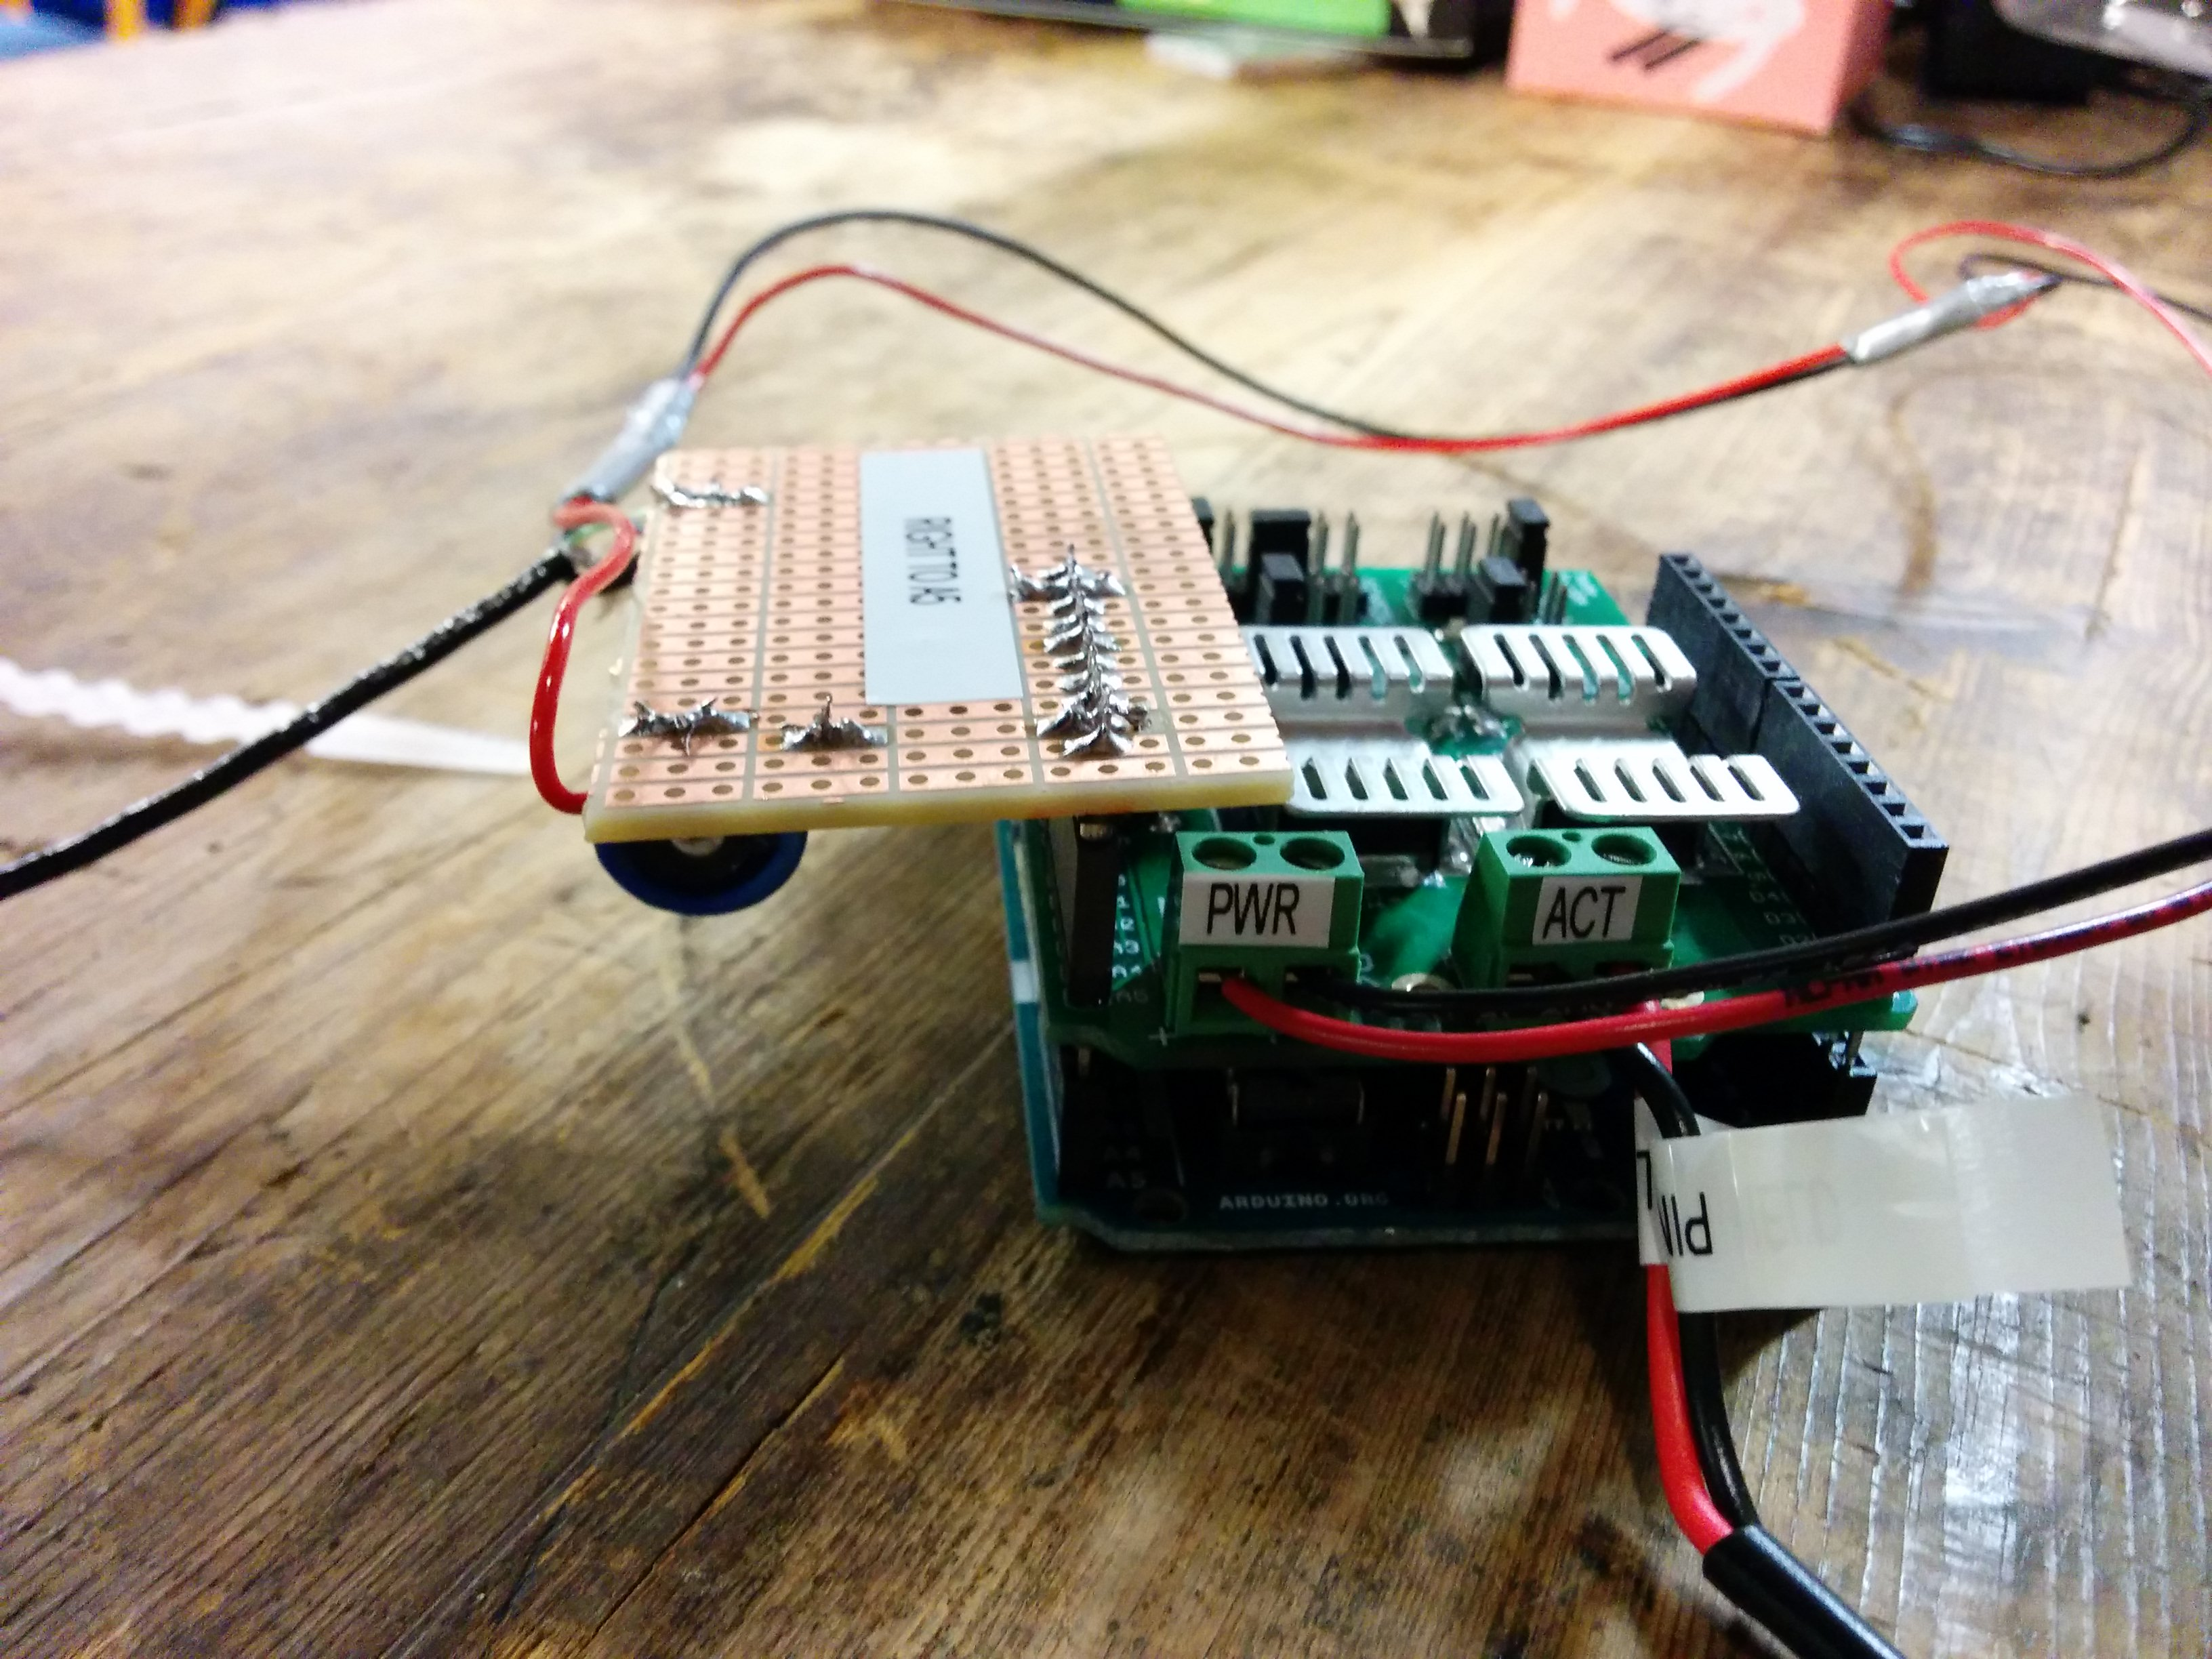
\includegraphics[width=.49\textwidth]{Figures/IMG_20150928_140547.jpg}
\caption{Connection of the Moto shield to the 12V power suppply and to the actuator.}
\end{center}
\end{figure}

\begin{figure}
\begin{center}
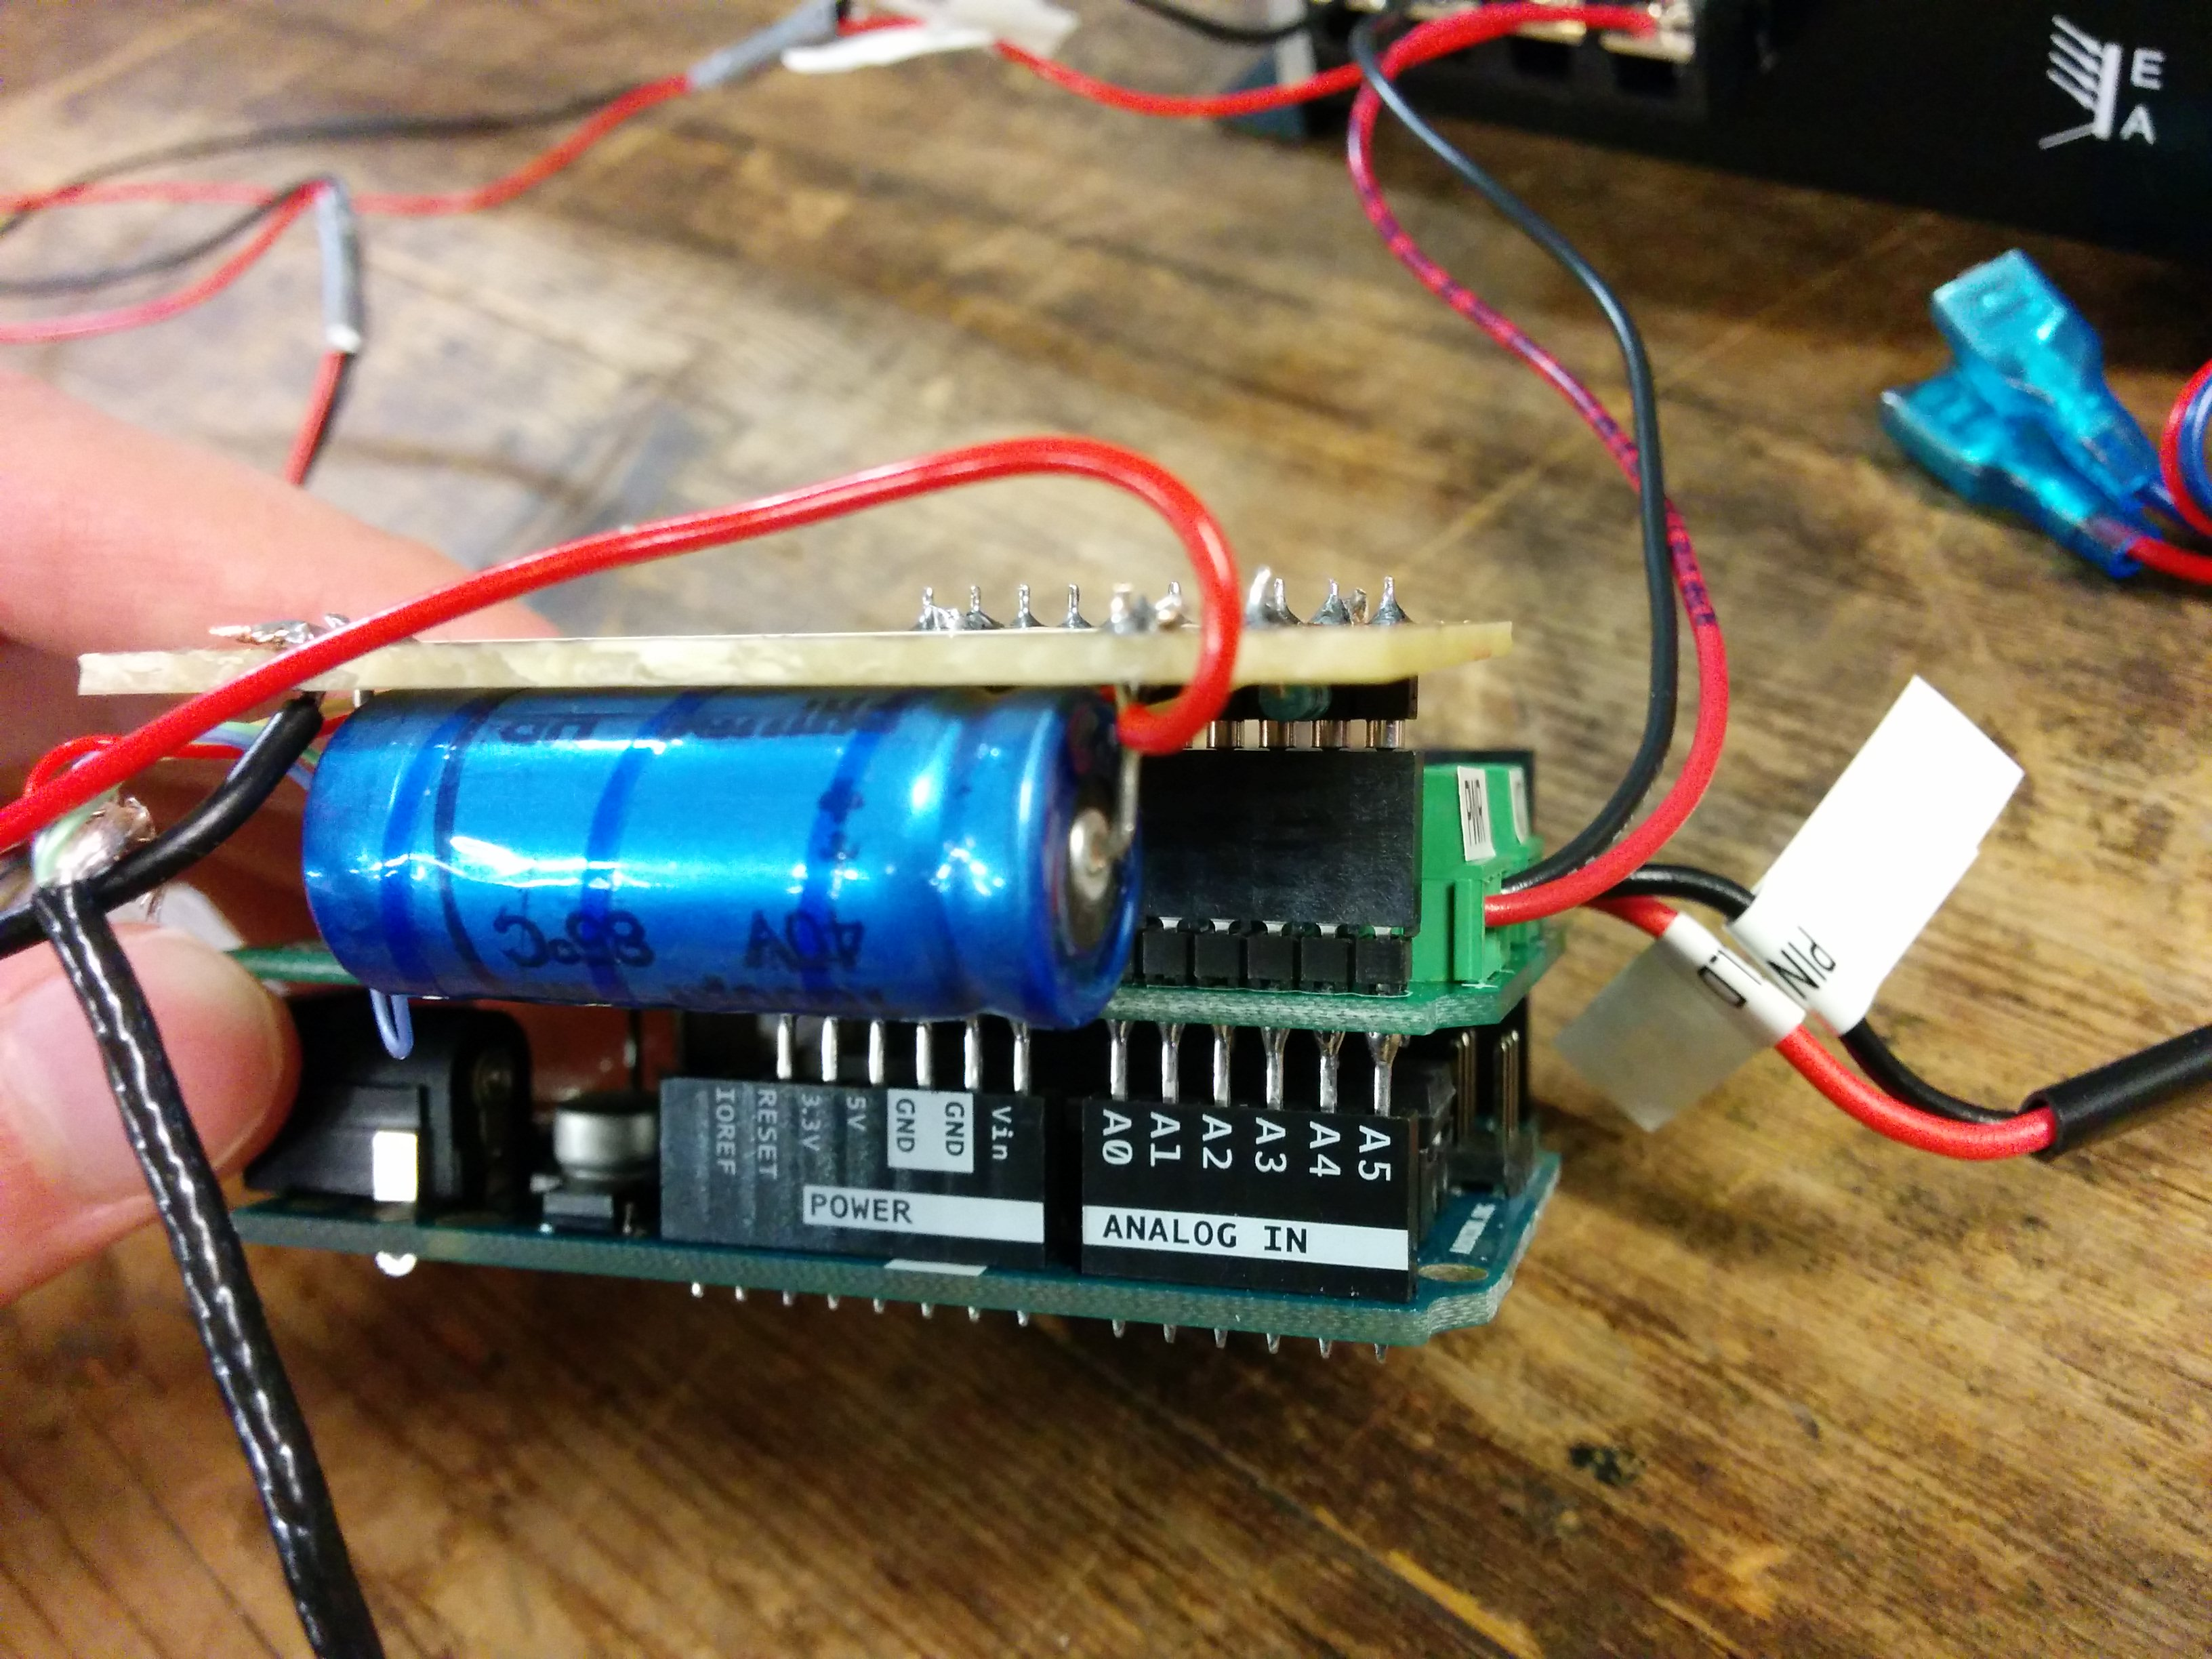
\includegraphics[width=.49\textwidth]{Figures/IMG_20150928_140626}
\caption{Connection of the soldered board on the Arduino through the Moto shield.}
\end{center}
\end{figure}

\begin{figure}
\begin{center}
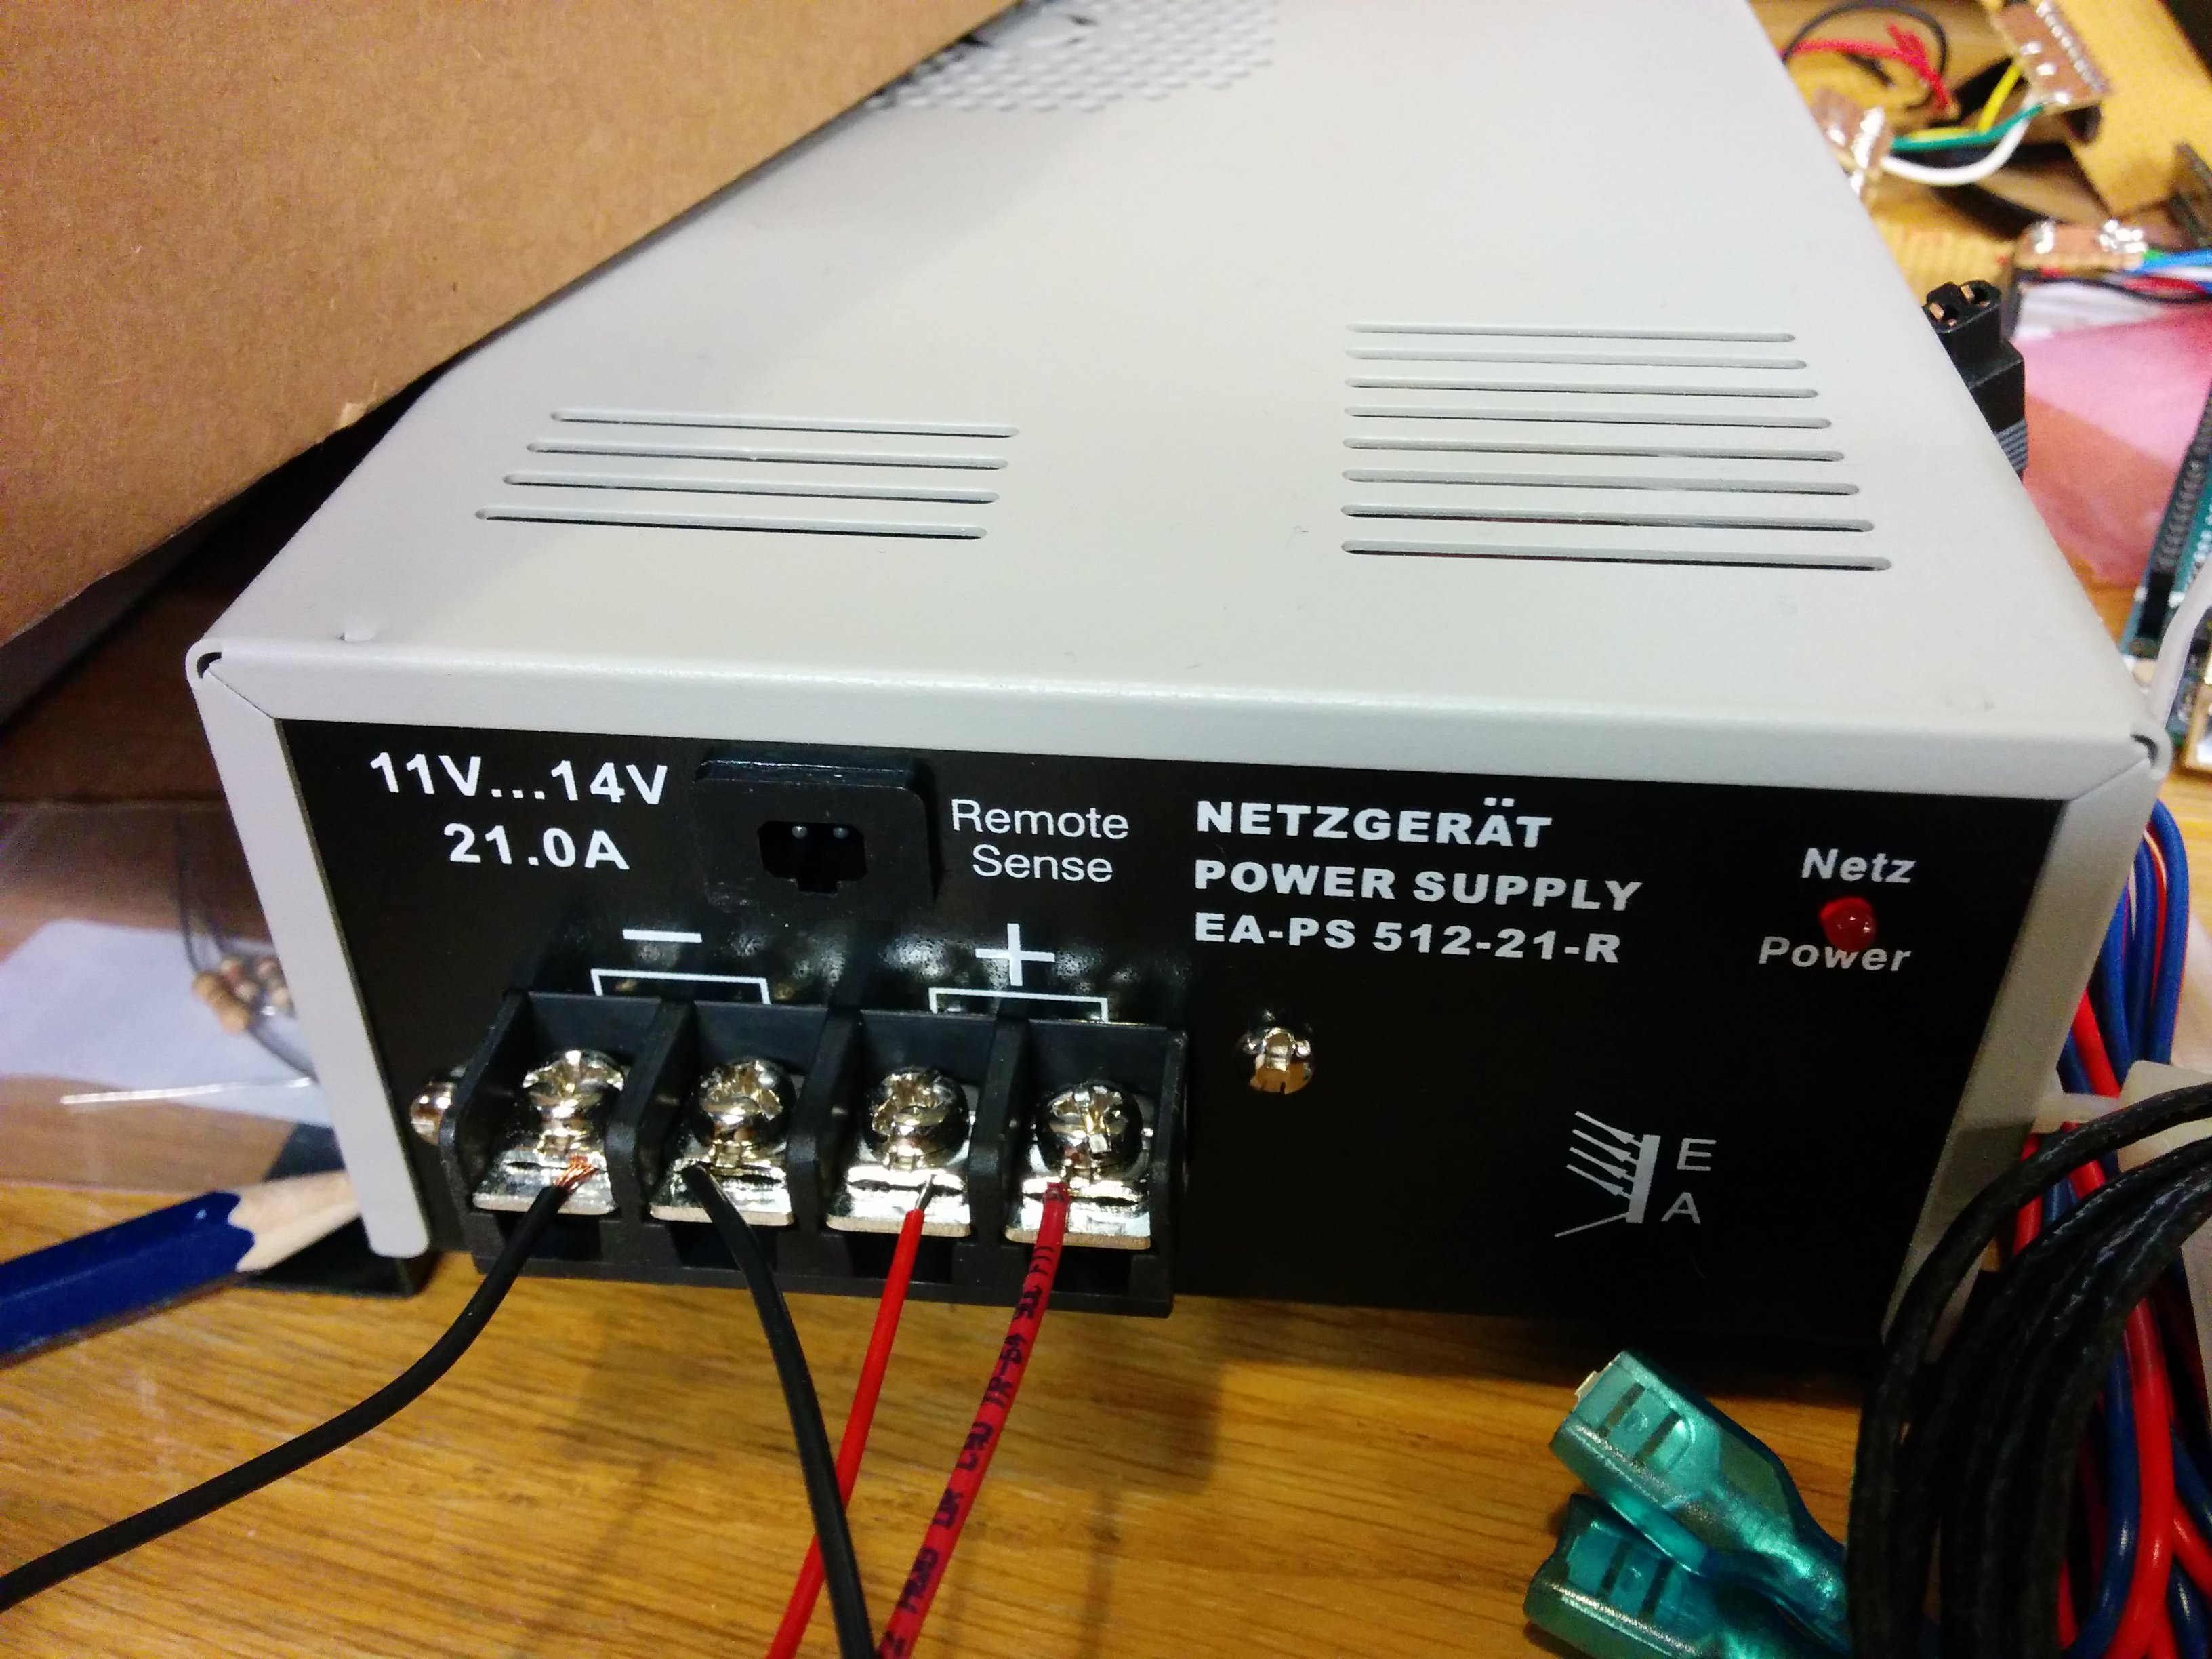
\includegraphics[width=.49\textwidth]{Figures/IMG_20150924_132227}
\caption{Connection of the power supply to both the Moto shield and the LVDT sensor on the 12V output.}
\end{center}
\end{figure}

\subsection{Physical configuration}

To test the system in the same configuration as used at UiO, the sensor should be held opposite to the actuator (see figure 4). If the relative orientation of the sensor and the actuator is changed, the Inv parameter must be changed also.

\begin{figure}
\begin{center}
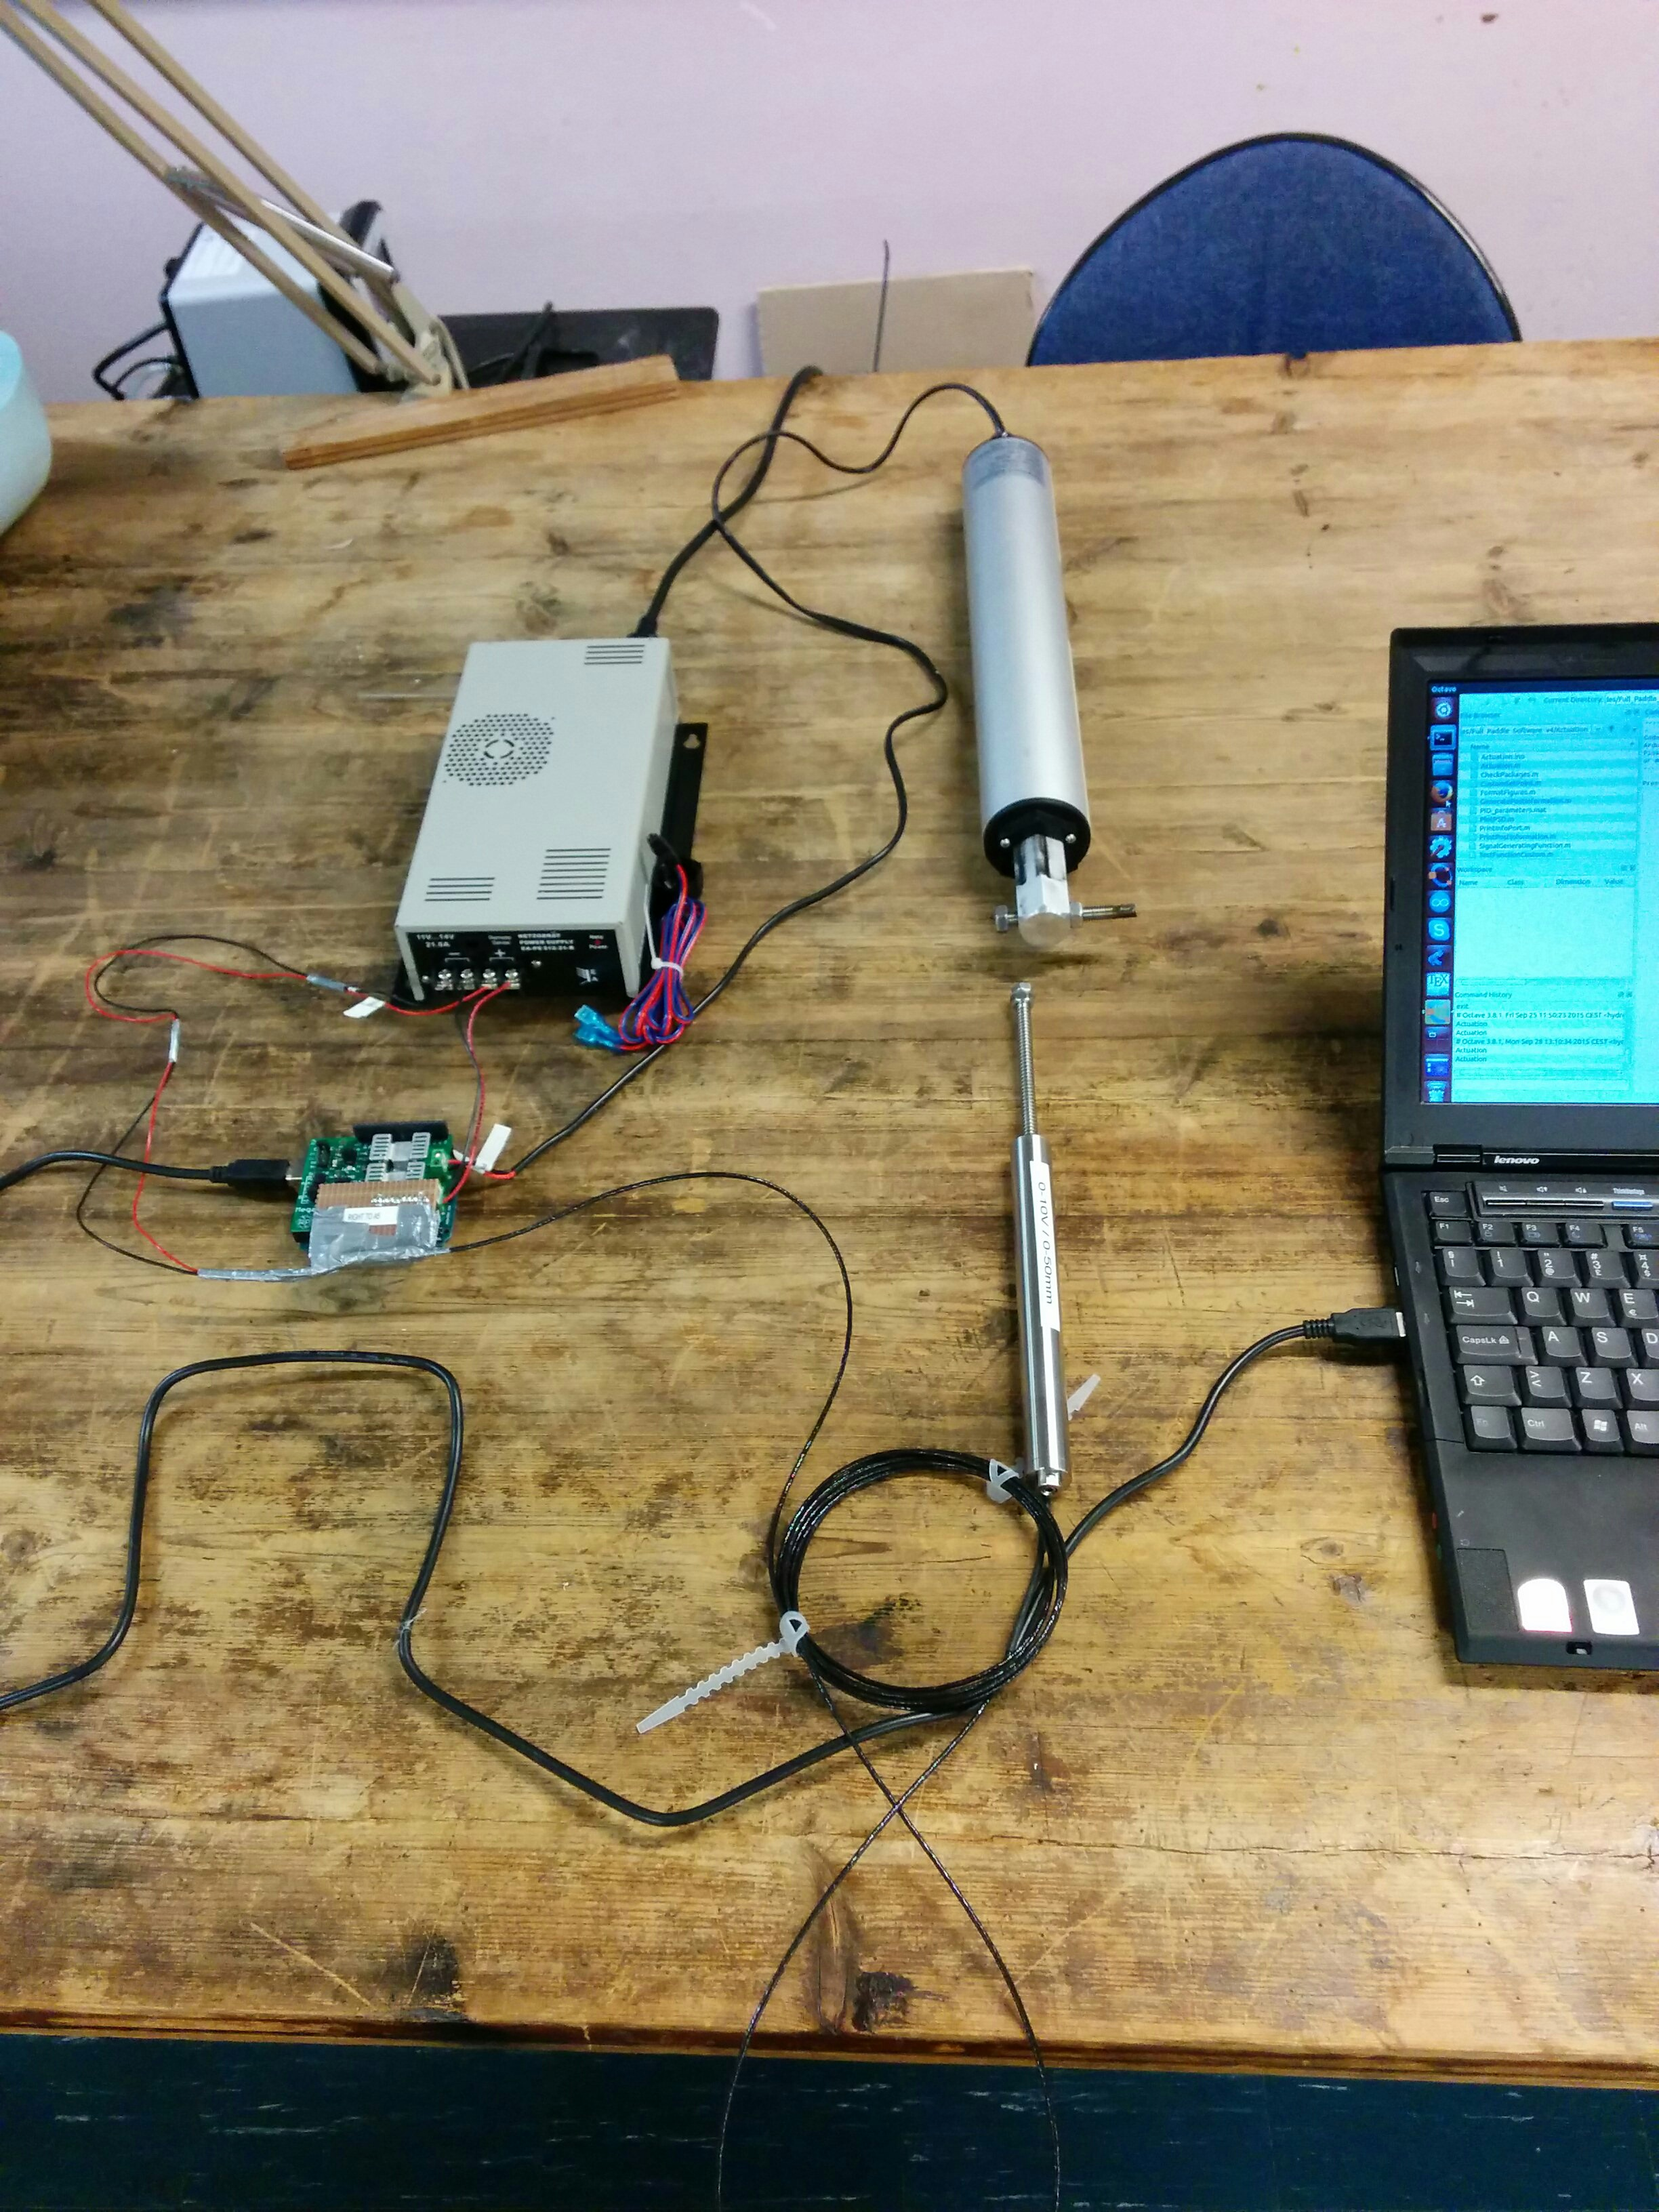
\includegraphics[width=.49\textwidth]{Figures/IMG_20150928_142209}
\caption{Physical configuration of the system, used at UiO for tests.}
\end{center}
\end{figure}

\subsection{Octave code}

The script is interactive and gives detailed instruction of the input needed at each step. The main steps are:

\begin{itemize}
\item Selection of the input signal, or re definition of the PID constants. Redefining the PID constants can be a way to try to optimize the paddle function. One should be careful about the choice of the coefficients to avoid unstable behaviour. In particular, the direction coefficient (Invert or Direct) should be selected with care to match the physical configuration. See section PID parameters tuning for more information. The history of the values chosen for the PID parameters is saved in PID\_parameters. By default, the latest set of parameters is used.
\item The default signals include monochromatic signal, modulated (two frequencies) signal, $tanh * sin$ signa and user defined signal. The signal 5 is a defautl 2 Hz sine, that can be used when testing for saving time.
\item Once the signal is selected, follow the instruction to fill up the required parameters. Once the parameters are chosen, the actuation will start. There is an approximately 5 seconds delay before the actuation starts, which is normal.
\item When the actuation has been performed, one can choose to analyse the data generated by the control system. This is useful to check the quality of the actuation. The information plotted corresponds to a full summary of the set point, true value and actuation control (figure 1 of the output), a zoomed comparison between set point and obtained position (figure 2 of the output), and an analysis of the PSD of the set point and obtained position (figure 3 of the output).
\item Finally, the script offers saving all the actuation data to a file, and to start a new actuation or quit the program
\end{itemize}

\subsection{PID parameters tuning}

The PID loop is controlled by three parameters $K_p$, $K_i$ and $K_d$. By convention, all three are taken positive. The command signal $C$ sent to the actuator is computed as:

$$ C(t) = Inv (K_p e(t) + K_i \int_{s=0}^{s=t} e(s) ds + \frac{d e}{dt} (t))$$

where $e(t)$ is the error between the set point $s$ and the measured position $p$, $e = s - p$. The $Inv$ parameter allows to take into account direct or indirect retroaction effect. If an increase of the command leads to a reduction of the error the $Inv$ parameter is 1 (Direct), in the countrary the $Inv$ parameter must be set to -1 (Indirect). If the $Inv$ parameter is wrong, the control system will be unstable. If the sytem is build as presented in figure FIG, using the default parameters, the control loop will be stable. If the polarity of the actuator input or the relative direction of the sensor to the actuator is changed, the $Inv$ parameter must be changed.

The choice of $K_p$, $K_i$ and $K_d$ depends on the actuator strength and inertia in the system. It can be adapted to the paddle by trial and error, checking the results using post actuation analysis in the reference case 5 for example. To tune the system, increase $K_p$ until the control loop starts to oscillate with both other parameters equal to zero. The good $K_p$ value should be taken approximately half of the unstable value. Once this good value is determined, increase $K_i$ will improve the control loop performance. Too high $K_i$ will lead to unstable control loop. Finally, increase $K_d$ will further improve the loop performance. Too high $K_d$ will lead to overshot.
 
\subsection{Troubleshooting}

\begin{itemize}
\item \emph{Problem connecting to the board:} The Octave programs searches the Arduino board on the ports /dev/ttyACM0 to /dev/ttyACM2. The boards needs a little bit of time to boot and be detected by the computer. If no board is detected, check that the board is powered (green LED on on the Arduino) and that the USB cable is used is adapted (for long distances), and try again. If the name of the port is different (should not be the case on Linux machines), change the ports name in the Octave code.
\item \emph{Unstable control system:} A bad choice of the PID parameters will lead to unstable control loop. The most critical parameter is the Inv parameter. Too high values of the other parameters can also lead to unstable control loop, see section ''PID Parameters Tuning'' for more details.
\item \emph{Bad position signal:} The LVDT probe uses magnetic inductance effects to perform the measurements. Electro Magnetic fields can disturb its good function. Do not place the LVDT probe on top of the actuator. If the probe is functionning well but the obtained position follows badly the set point, try to reduce signal amplitude and \/ or signal frequency. The actuator has limited performance, and asking for too high amplitude \/ frequencies will saturate the actuator command (saturated command can be checked by performing the post actuation analysis).
\end{itemize}

\section{System test}

Results obtained at UiO, using the PID tuning parameters loaded in the Octave code and the physical configuration of figure 4, are presented in figures 5 and 6.

\begin{figure}
\begin{center}
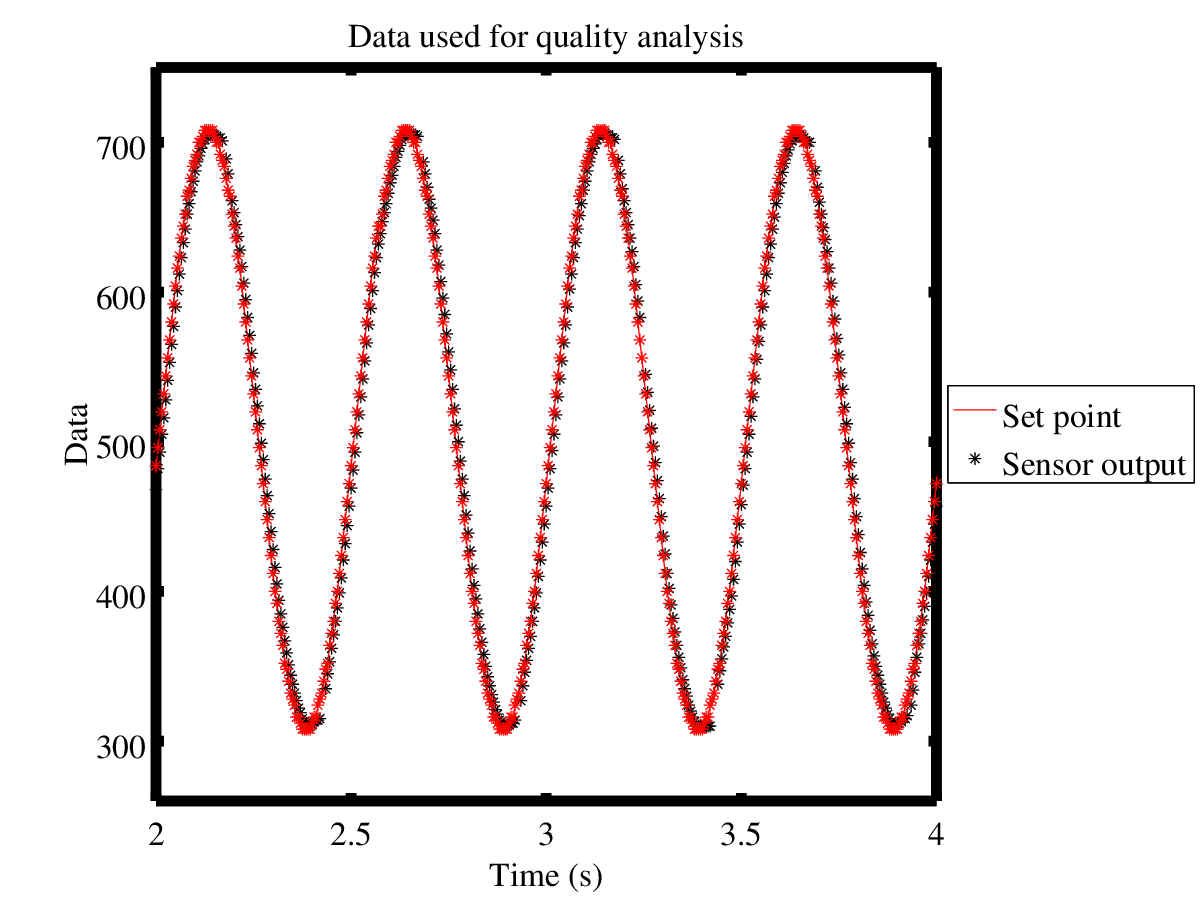
\includegraphics[width=.49\textwidth]{Figures/Sine2Hz_test2.png}
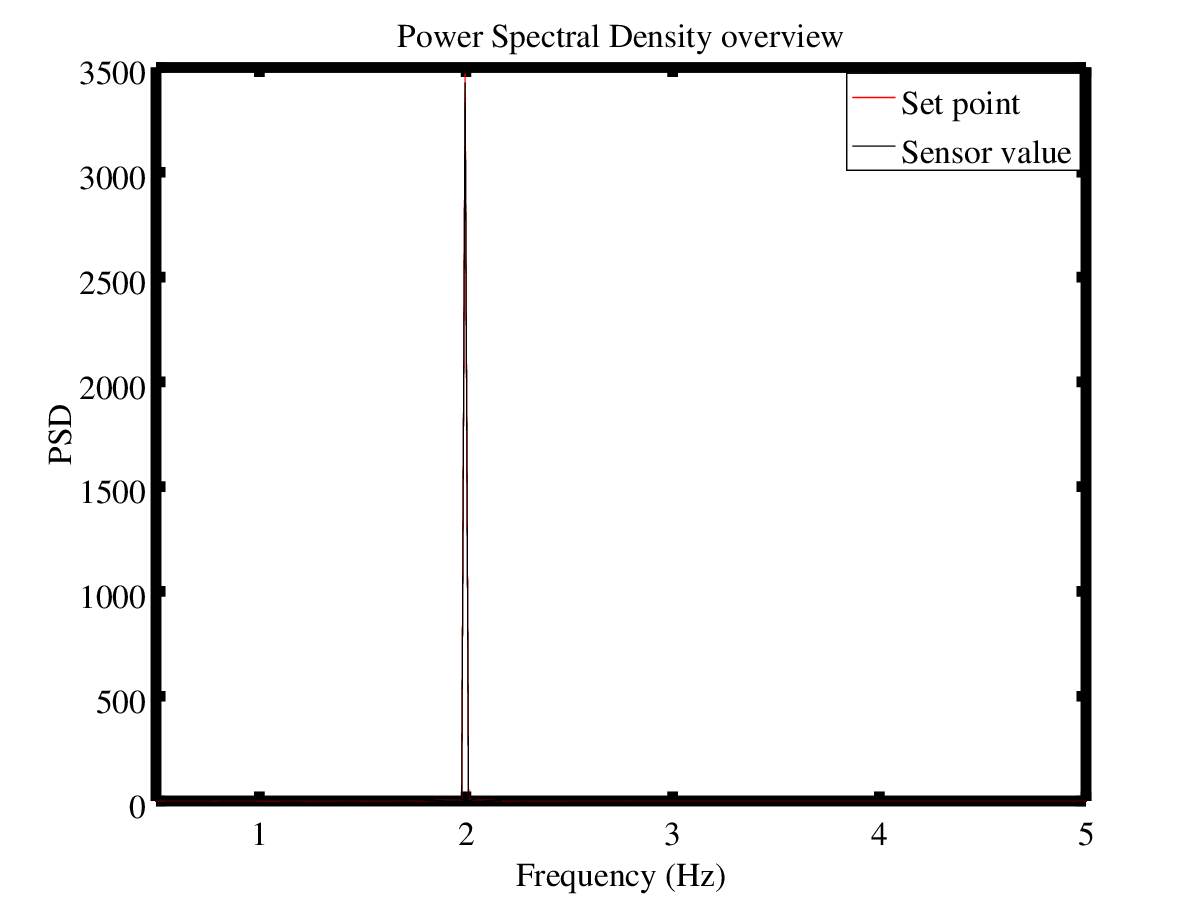
\includegraphics[width=.49\textwidth]{Figures/PSD_2HzSine_test2.png}
\caption{Performance test, 2Hz control signal. Data on Y-Axis of left figure is read from the 10 bits Arduino ADC, full range 0 - 1023 corresponds to 50 mm. Rigth figure: spectral content of the set point and obtained position.}
\end{center}
\end{figure}

\begin{figure}
\begin{center}
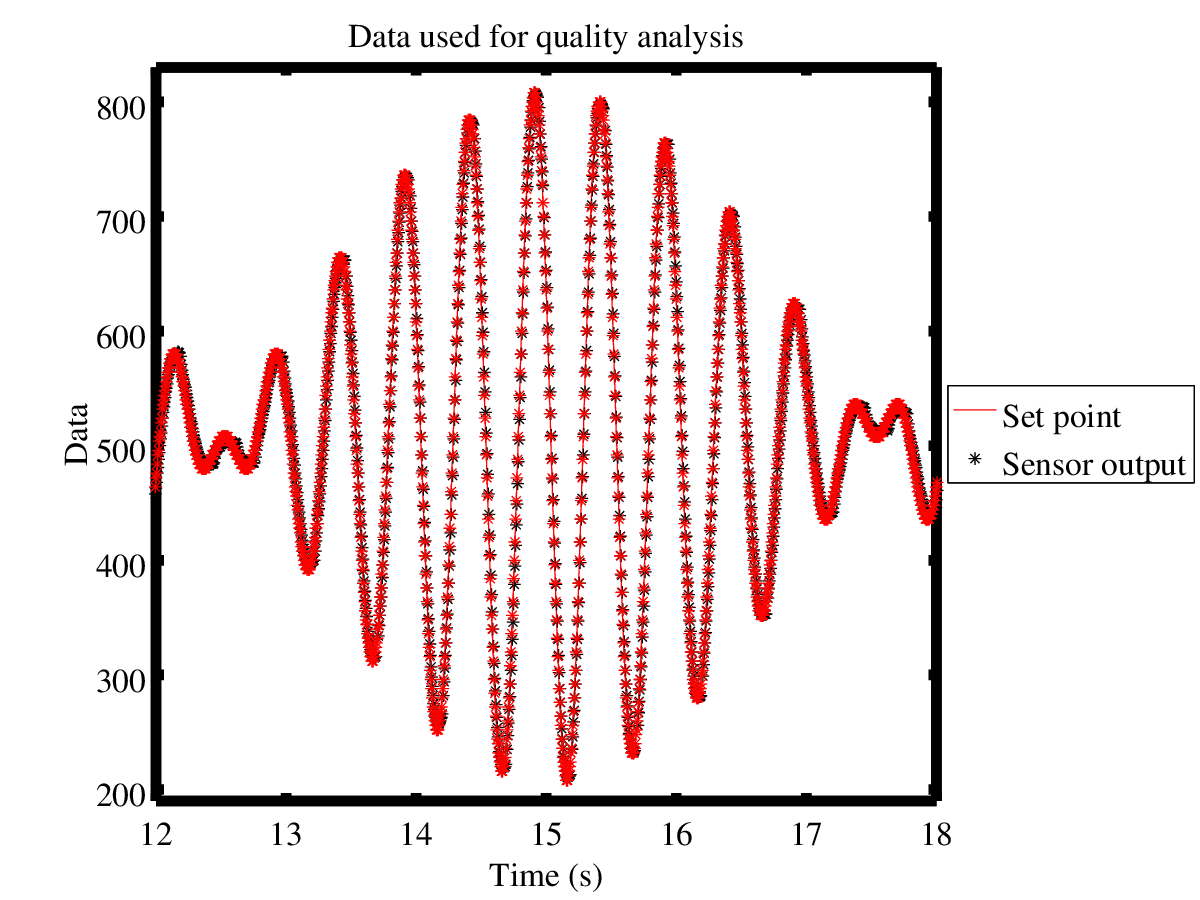
\includegraphics[width=.5\textwidth]{Figures/ModulatedSine_test1.png}
\caption{Test using a modulated sinusoid. Data is indicated as 10 bits from Arduino ADC.}
\end{center}
\end{figure}

\end{document}